\documentclass{beamer}

\usetheme{metropolis}
\usepackage{appendixnumberbeamer}

\usepackage{transparent}
\usepackage[english]{babel}
\usepackage[sfdefault]{FiraSans}
\usepackage{amssymb,mathrsfs,mathtools}
\usepackage{amsfonts}
\usepackage{tikz,pgfopts,etoolbox,calc,ifxetex,ifluatex}
\usepackage{subcaption}
\usefonttheme[onlymath]{serif}

\newcommand\independent{\protect\mathpalette{\protect\independenT}{\perp}}
\def\independenT#1#2{\mathrel{\rlap{$#1#2$}\mkern2mu{#1#2}}}
\let\oldemptyset\emptyset
\let\emptyset\varnothing

\setbeamercovered{highly dynamic}

\title{\textsc{A Bayesian model for data flow: BikeMi}}
\subtitle{}
\author{Andrea De Gobbis, Lorenzo Ghilotti, Giorgio Meretti}
\institute{Politecnico di Milano}
\logo{\includegraphics[width=15mm]{Politecnico_di_Milano}}
\date{February 19, 2020}
\usetheme{Goettingen}
\usecolortheme{dolphin}

\begin{document}

\begin{frame}
 \maketitle
\end{frame}

\begin{frame}{What we are working on}

The BikeMi stations net in Milan is rather large and travelled every day.
\begin{figure}[H]
\centering
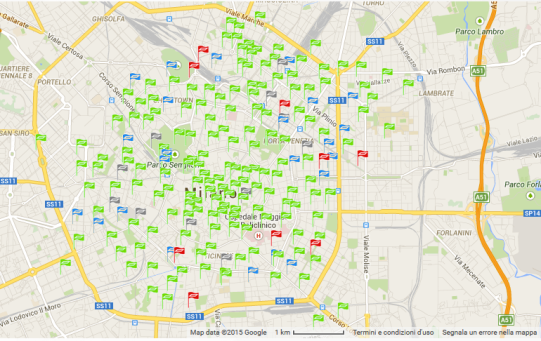
\includegraphics[width=1\linewidth]{pictures/mappa.png} 
\end{figure}

\end{frame}

\begin{frame}{The two perspective of the problem}
	Our work is structured in two parts:

\vspace{5mm}

\begin{columns}

\begin{column}{.5\textwidth}

	\alert{Global model} \\
The total volume of travels in a specific day $Y_t$ without considering the graph structure. This results in a single time series.

\end{column}

\hspace{5pt}

\vrule{}

\hspace{8pt}

\begin{column}{.5\textwidth}
	
	\alert{Network model}\\
For each node, the analysis focuses on in and out bikes flow for specific time slots. The dimensionality is much higher.
	
\end{column}

\end{columns}
\end{frame}

\begin{frame}{Loglinear GLM: Poisson likelihood}
\begin{equation*}
\begin{aligned}
&\textsc{Model}\\
&Y_t  |  \lambda_t \overset{ind}{\sim} \mathrm{Po}(\lambda_t)\\
&\log{\lambda_t} = \boldsymbol{\beta}^T\mathbf{z}_t\\
\end{aligned}
\qquad \qquad
\begin{aligned}[c]
&\textsc{Prior}\\
&\beta_i \overset{iid}{\sim}\mathcal{N}(0,\sigma^2_\beta)\\
&\\
\end{aligned}
\end{equation*}
\end{frame}

\begin{frame}{Loglinear GLM: Poisson likelihood}
\begin{figure}[H]
\centering
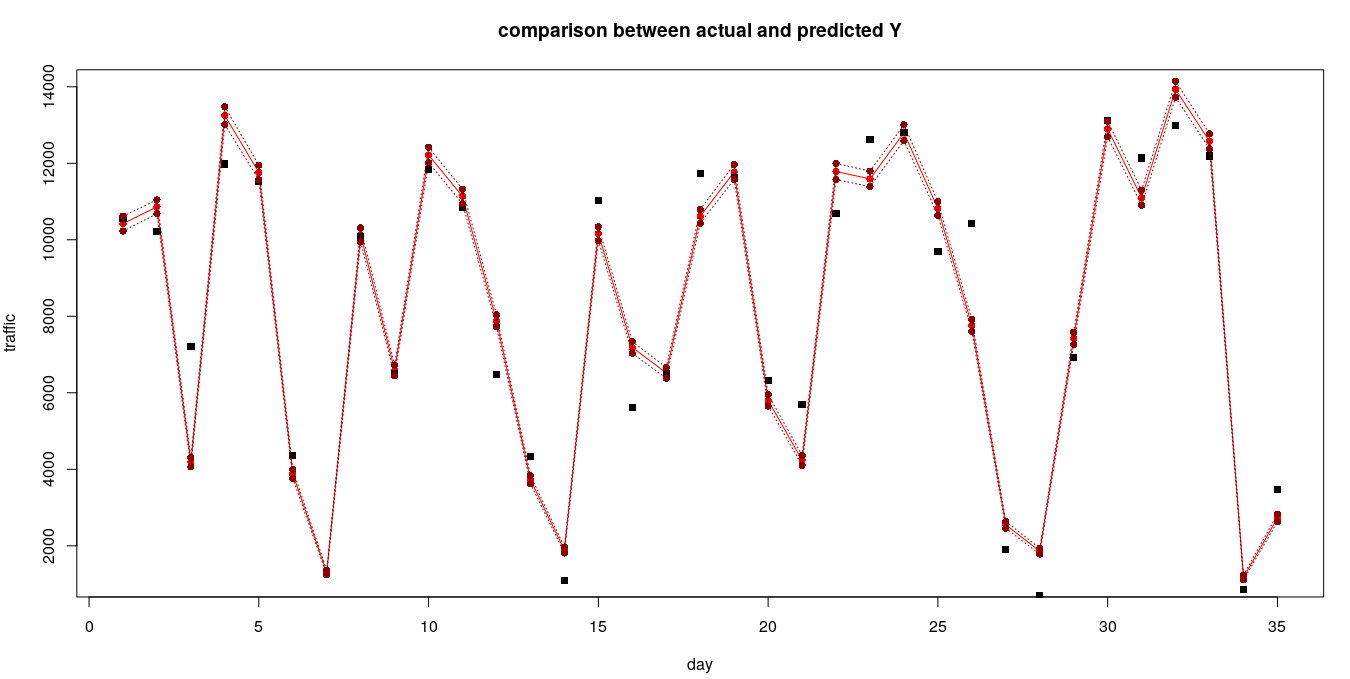
\includegraphics[width=1\linewidth]{pictures/poiss_y.png} 
\end{figure}
\end{frame}

\begin{frame}{Negative Binomial distribution}
$$X \sim \mathrm{NegBin}(p,r) \ if:$$
$$f(k;p,r) = \frac{\Gamma(k+r)}{k!\Gamma(r)} p^k (1-p)^r, \qquad k = 0,1,2...$$
$$\mathbb{E}[X] = \mu = \frac{r(1-p)}{p} \qquad Var(X) = \frac{r(1-p)}{p^2}$$
Moreover:
$$p = \frac{r}{r+\mu}$$
\end{frame}

\begin{frame}{Loglinear GLM: NegBin likelihood (1)}
\begin{equation*}
\begin{aligned}
&\textsc{Model}\\
&Y_t | p_t,r \overset{ind}{\sim} \mathrm{NegBin}(p_t,r)\\
&p_t = \frac{r}{r+\mu_t}\\
&\log{\mu_t} = \boldsymbol{\beta}^T\mathbf{z}_t\\
\end{aligned}
\qquad \qquad
\begin{aligned}[c]
&\textsc{Priors}\\
&\boldsymbol{\beta} \sim \mathcal{N}_p(\mathbf{0}, \sigma^2_\beta\mathbf{I})\\
&r \sim \mathcal{U}(0,50)\\
&\\
\end{aligned}
\end{equation*}
\end{frame}

\begin{frame}{Loglinear GLM: NegBin likelihood (1)}
\begin{figure}[H]
\centering
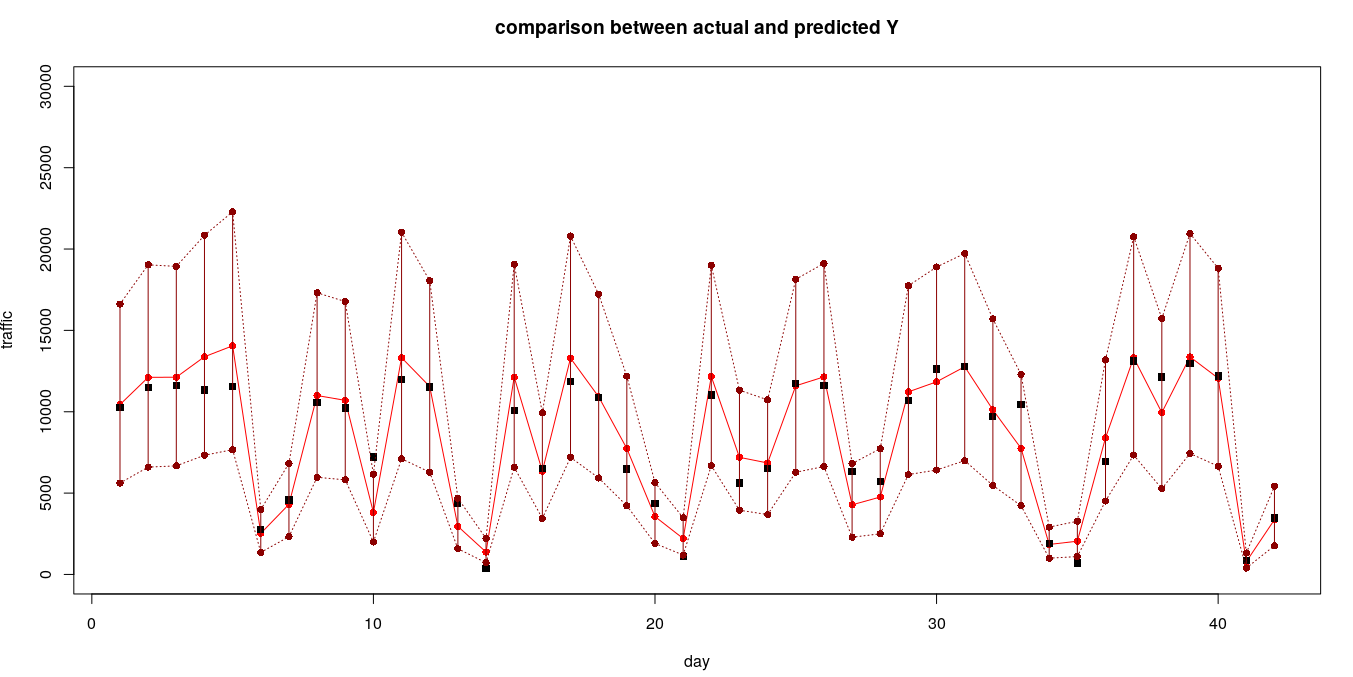
\includegraphics[width=1\linewidth]{pictures/negbin_single_r_pred.png} 
\end{figure}
\end{frame}

\begin{frame}{Loglinear GLM: NegBin likelihood (2)}
\begin{equation*}
\begin{aligned}
&\textsc{Model}\\
&Y_{tj}  |  p_{tj},r_j \overset{ind}{\sim} \mathrm{NegBin}(p_{tj},r_j) \qquad j = 1: wday, j = 2: wend\\
&p_{tj} = \frac{r_j}{r_j + \mu_{tj}}\\
&\log{\mu_{tj}} = \beta_1 + \beta_2R_{t} + \beta_3T_{t} + \theta_j\\
&\textsc{Priors}\\
&\beta_i | \tau_i \overset{ind}{\sim} \mathcal{N}(0, \tau_i) \ i = 1,2,3\\
&\tau_i \overset{ind}{\sim} Gamma(2,10) \\
&\theta_j | \tilde{\tau}_j \overset{ind}{\sim} \mathcal{N}(0, \tilde{\tau}_j) \ j = 1,2\\
&\tilde{\tau}_j \overset{ind}{\sim} Gamma(2,10)\\
&r_j \overset{ind}{\sim} Unif(0,50) \ j = 1,2\\
\end{aligned}
\end{equation*}
\end{frame}

\begin{frame}{Loglinear GLM: NegBin likelihood (2)}
\begin{figure}[H]
\centering
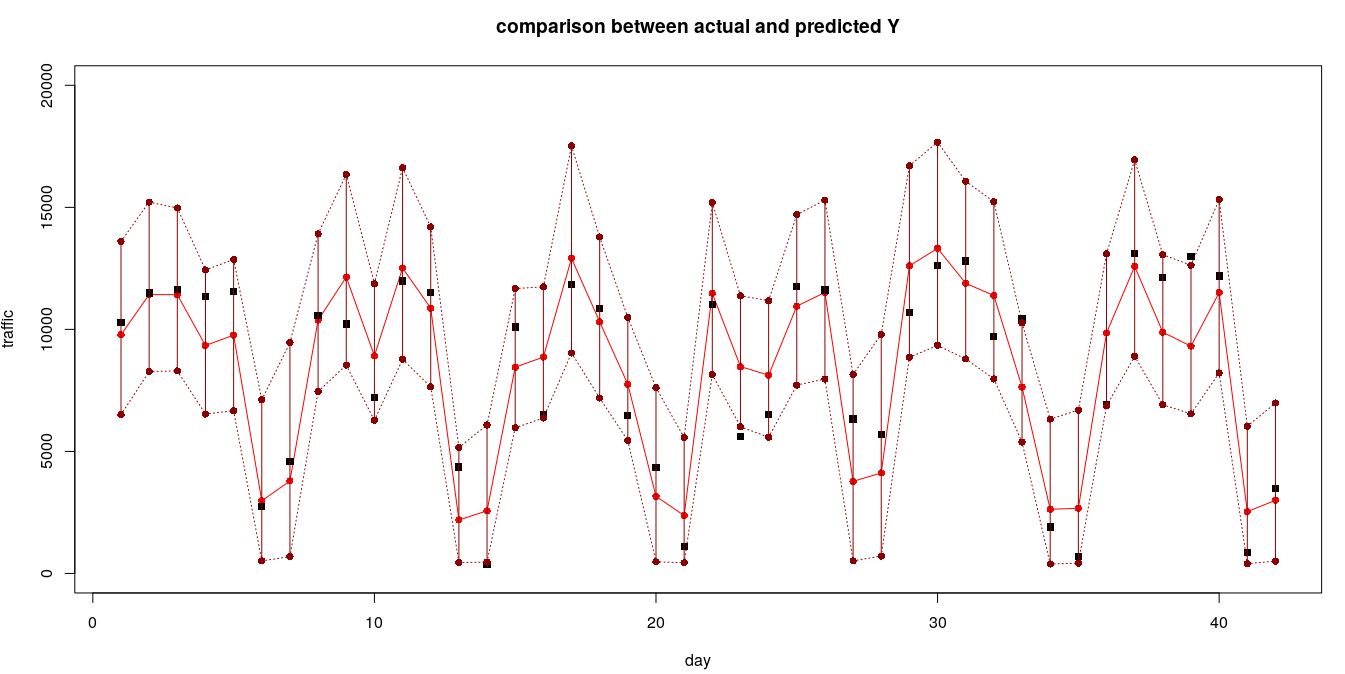
\includegraphics[width=1\linewidth]{pictures/negbin_double_r_pred.png} 
\end{figure}
\end{frame}

\begin{frame}{Ingredients of a BSTS}
\begin{figure}[H]
	Main ingredients of \alert{BSTS} model:
	\begin{itemize}
		\item locally linear trend \alert{$ \mu_t $},
		\transparent{0.25}
		{
		\item periodicity \alert{$ \gamma_t $},
		\item autoregressive component \alert{$ \rho_t $},
		\item regression \alert{$ \boldsymbol{\beta}^T\mathbf{z} $}.
		} 
	\end{itemize}
\end{figure}
\end{frame}

\begin{frame}{Ingredients of a BSTS}
\begin{figure}[H]
	Main ingredients of \alert{BSTS} model:
	\begin{itemize}
		\item locally linear trend \alert{$ \mu_t $},
		\item periodicity \alert{$ \gamma_t $},
				\transparent{0.25}
		{
			\item autoregressive component \alert{$ \rho_t $},
			\item regression \alert{$ \boldsymbol{\beta}^T\mathbf{z} $}.
		} 
	\end{itemize}
\end{figure}
\end{frame}

\begin{frame}{Ingredients of a BSTS}
\begin{figure}[H]
	Main ingredients of \alert{BSTS} model:
	\begin{itemize}
		\item locally linear trend \alert{$ \mu_t $},
		\item periodicity \alert{$ \gamma_t $},
		\item autoregressive component \alert{$ \rho_t $},
				\transparent{0.25}
		{
			\item regression \alert{$ \boldsymbol{\beta}^T\mathbf{z} $}.
		} 
	\end{itemize}
\end{figure}
\end{frame}

\begin{frame}{Ingredients of a BSTS}
\begin{figure}[H]
	Main ingredients of \alert{BSTS} model:
	\begin{itemize}
		\item locally linear trend \alert{$ \mu_t $},
		\item periodicity \alert{$ \gamma_t $},
		\item autoregressive component \alert{$ \rho_t $},
		\item regression \alert{$ \boldsymbol{\beta}^T\mathbf{z} $}.
	\end{itemize}
\end{figure}
\end{frame}


\begin{frame}{Standard BSTS}
\tiny

\begin{equation*}
	\begin{aligned}
&\textsc{Model}\\
&Y_t = \mu_t + \gamma_t + \rho_t + \boldsymbol{\beta}^T\mathbf{z}_t + \tau_\epsilon^{-\frac{1}{2}}\tilde{\epsilon}_t\\
&\mu_t = \mu_{t-1} + \delta_{t-1} +\tau_\eta^{-\frac{1}{2}}\tilde{\eta}_t\\
&\delta_t = \delta_{t-1} + \tau_v^{-\frac{1}{2}}\tilde{v}_t\\
&\gamma_t = \sum_{i=1}^{S-1}\gamma_{t+i-S} + \tau_w^{-\frac{1}{2}}\tilde{w}_t\\
&\rho_t = \alpha\rho_{t-1} + \tau_u^{-\frac{1}{2}}\tilde{u}_t\\
&\tilde{\epsilon}_t, \tilde{\eta}_t, \tilde{v}_t, \tilde{w}_t, \tilde{u}_t \overset{iid}{\sim} \mathcal{N}(0,1)\\
\\
&\textsc{Initial Conditions}\\
&\mu_0 \sim \mathcal{N}(m, \tau_\eta)\quad \quad\quad\quad \quad \quad \quad\  m\ \ hpm\\
&\delta_0 \sim \mathcal{N}(d, \tau_v)\quad\quad\quad\quad \quad \quad \quad \quad d\ \ \ hpm\\
&\boldsymbol{\gamma}_{0:(2-S)} \sim \mathcal{N}_{S-1}(\mathbf{g}, \tau_w\mathbf{I})\quad\ \ \mathbf{g}\ \ hpm\\
&\rho_0 \sim \mathcal{N}(r, \tau_u)\quad \quad\quad\quad \quad \quad \quad \quad \ r\ \ hpm\\
\\
\end{aligned}
\qquad \qquad
\begin{aligned}[c]
&\textsc{Priors}\\
&\boldsymbol{\beta} \sim \mathcal{N}_p(\mathbf{0}, \tau_b \mathbf{I})\ \ \quad \quad \quad \quad \quad \tau_b\ \quad \ hpm\\
&\alpha \sim \mathcal{N}(a, \tau_a) \ \quad \quad \quad \quad \quad \quad a, \tau_a\ \ hpm\\
&\tau_\epsilon \sim Unif(a_\epsilon, b_\epsilon)\quad\quad\ \quad \quad a_\epsilon, b_\epsilon\ \ hpm\\
&\tau_\eta \sim Unif(a_\eta, b_\eta)\quad\quad\quad \quad a_\eta, b_\eta\ \ hpm\\
&\tau_v \sim Unif(a_v, b_v)\quad\quad\quad \quad a_v, b_v\ \ hpm\\
&\tau_w\sim Unif(a_w, b_w)\quad\quad\quad\ a_w, b_w\ \ hpm\\
&\tau_u \sim Unif(a_u, b_u)\quad\quad\quad\quad a_u, b_u\ \ hpm\\
&\\
&\\
&\\
&\textsc{Independence}\\
&\{\tilde{\epsilon}_t, \tilde{\eta}_t, \tilde{u}_t, \tilde{w}_t, \tilde{v}_t, \mu_0, \delta_0, \boldsymbol{\gamma}_{0:(-S+2)}, \rho_0,\\ &\boldsymbol{\beta}, \alpha, \tau_\epsilon, \tau_\eta, \tau_v, \tau_w, \tau_u\}\\ &family\ of\ \independent real\ random\ variables\\
&\\
&\\
\end{aligned}
\end{equation*}
\end{frame}

\begin{frame}{Hyperparameters for  BSTS}
We fix the \alert{hyperparameters} as follows:
\begin{table}[!htb]
	\centering
		\begin{tabular}{|c|c|c|c|c|c|}
			\hline
			& $ \tau_\epsilon $ & $ \tau_\eta $ &$  \tau_v $ & $ \tau_w $ & $ \tau_ u $\\
			\hline
			a &$  1\mathrm{e}{-7} $ & $  1\mathrm{e}{-5} $ &$  1\mathrm{e}{-5} $&$  1\mathrm{e}{-5} $&$  1\mathrm{e}{-5} $\\
			\hline
			b &$  1\mathrm{e}{-4} $ & $  1\mathrm{e}{-4} $ &$  1\mathrm{e}{-4} $&$  1\mathrm{e}{-4} $&$  1\mathrm{e}{-3} $\\
			\hline
		\end{tabular} 
\end{table}

$ m $ and $ \mathbf{g} $ according to \alert{frequentist stationarization}

\begin{table}[!htb]
	\centering
		\begin{tabular}{|c|c|c|c|c|}
			\hline
			& $ \tau_\alpha $ & $ \tau_\beta $ & $ r $ & $ d $\\
			\hline
			value &$  1\mathrm{e}{-5} $ & $  1\mathrm{e}{-5} $& 0 & 0\\
			\hline
		\end{tabular} 
\end{table}
\end{frame}

\begin{frame}{4 rules for a proper evaluation}
\begin{enumerate}
	\item performance is subject to correctness of modelling assumptions and \alert{proper diagnostics},
	\item use codified Beyesian tools to evaluate the worth of a model from a \alert{predictive} viewpoint,
	\item in absence of strong evidence for a format let \alert{interpretability} be the deciding factor,
	\item in case of a draw in the previous points, select the \alert{simplest} paradigm.
\end{enumerate}
\end{frame}

\begin{frame}{Some diagnostics}
\begin{figure}[H]
		\centering
		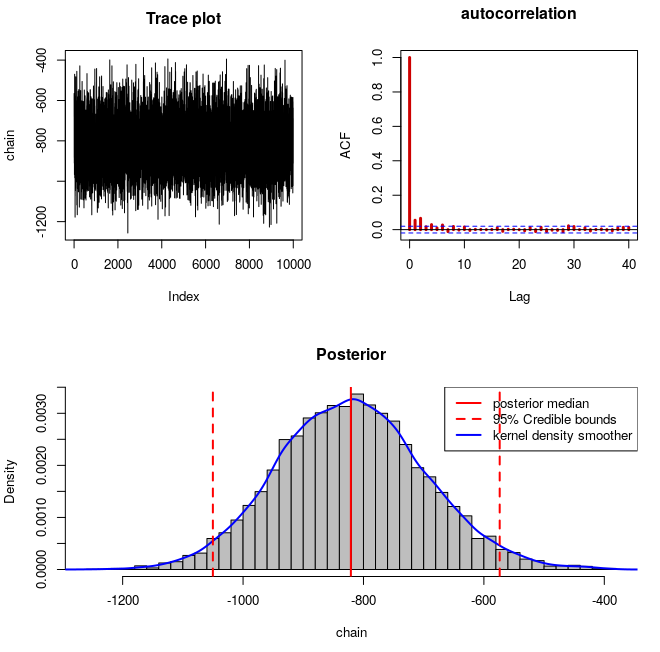
\includegraphics[width=60 mm]{pictures/beta_1.png}
		\caption{\tiny Diagnostics for $ \beta_1 $ samples}
		\label{fig:beta_1}
\end{figure}
\end{frame}


\begin{frame}{Prediction}
\begin{figure}[H]
	\centering
	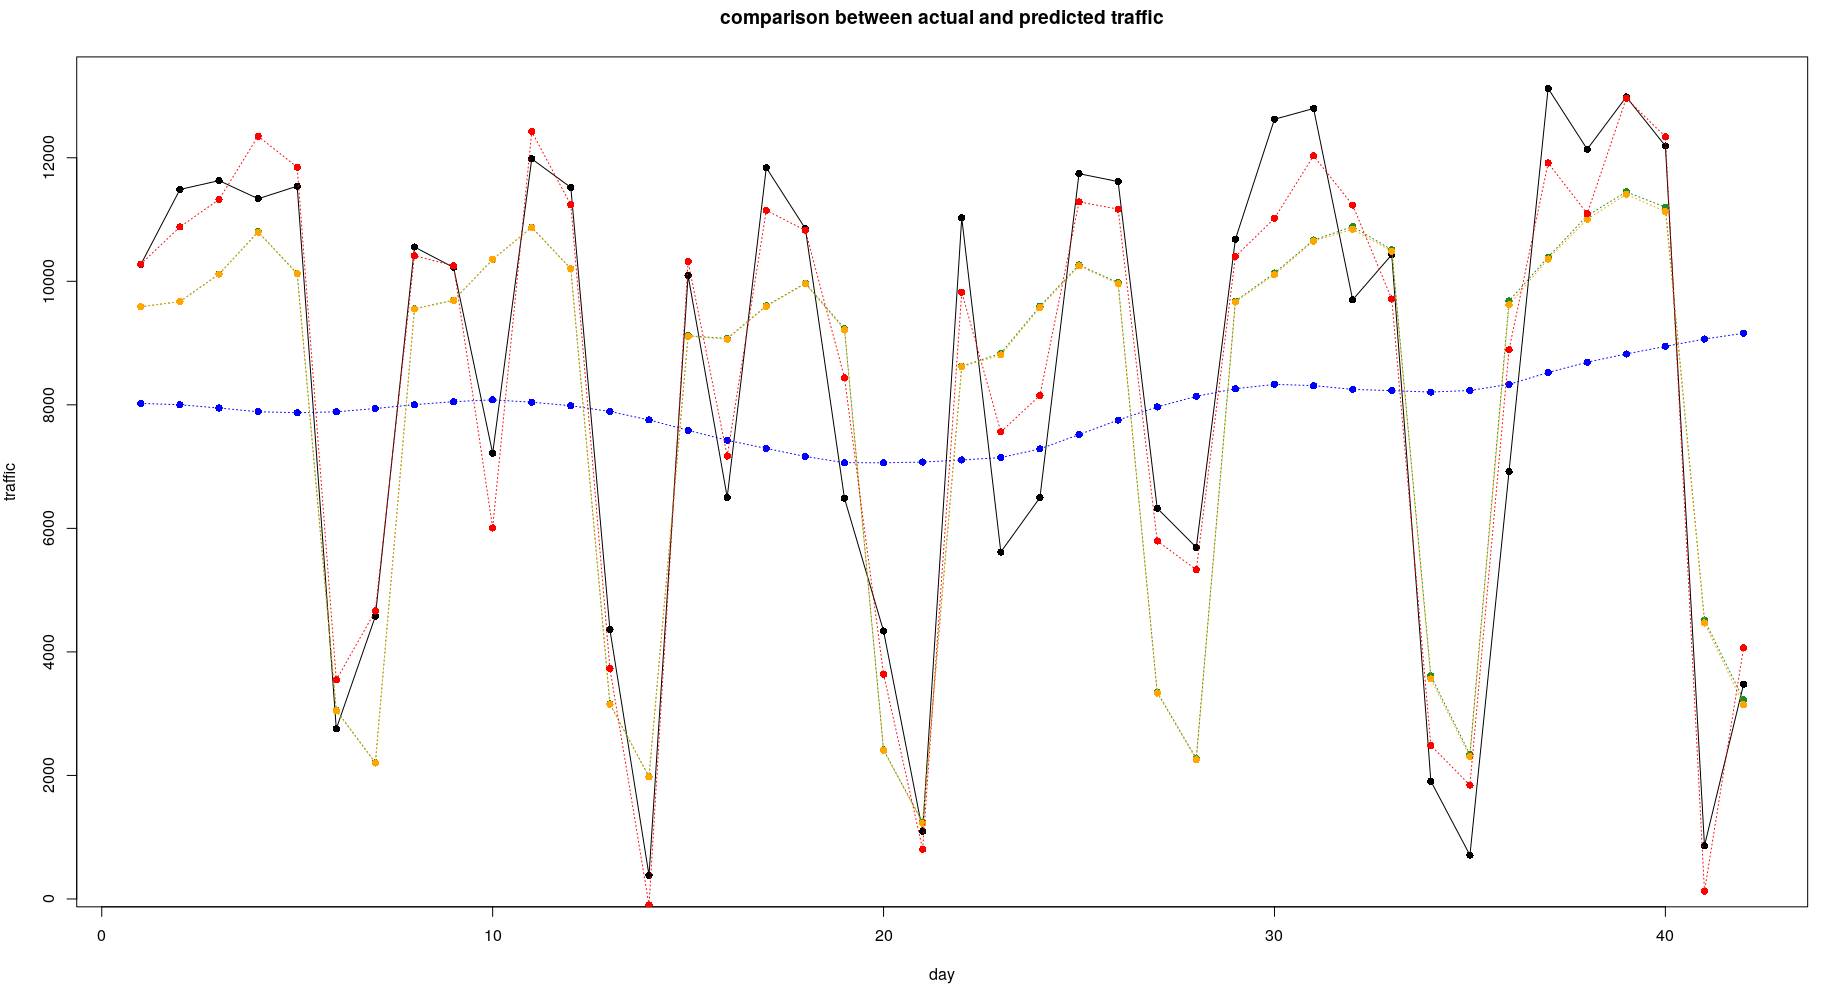
\includegraphics[width=100 mm]{pictures/m2_g1.png}
	\caption{Sum of trend (blue), periodicity (green), autoregression (yellow) and regression (red)}
	\label{fig:M2_p1}
\end{figure}
\end{frame}

\begin{frame}{Prediction}
\begin{figure}[H]
	\centering
	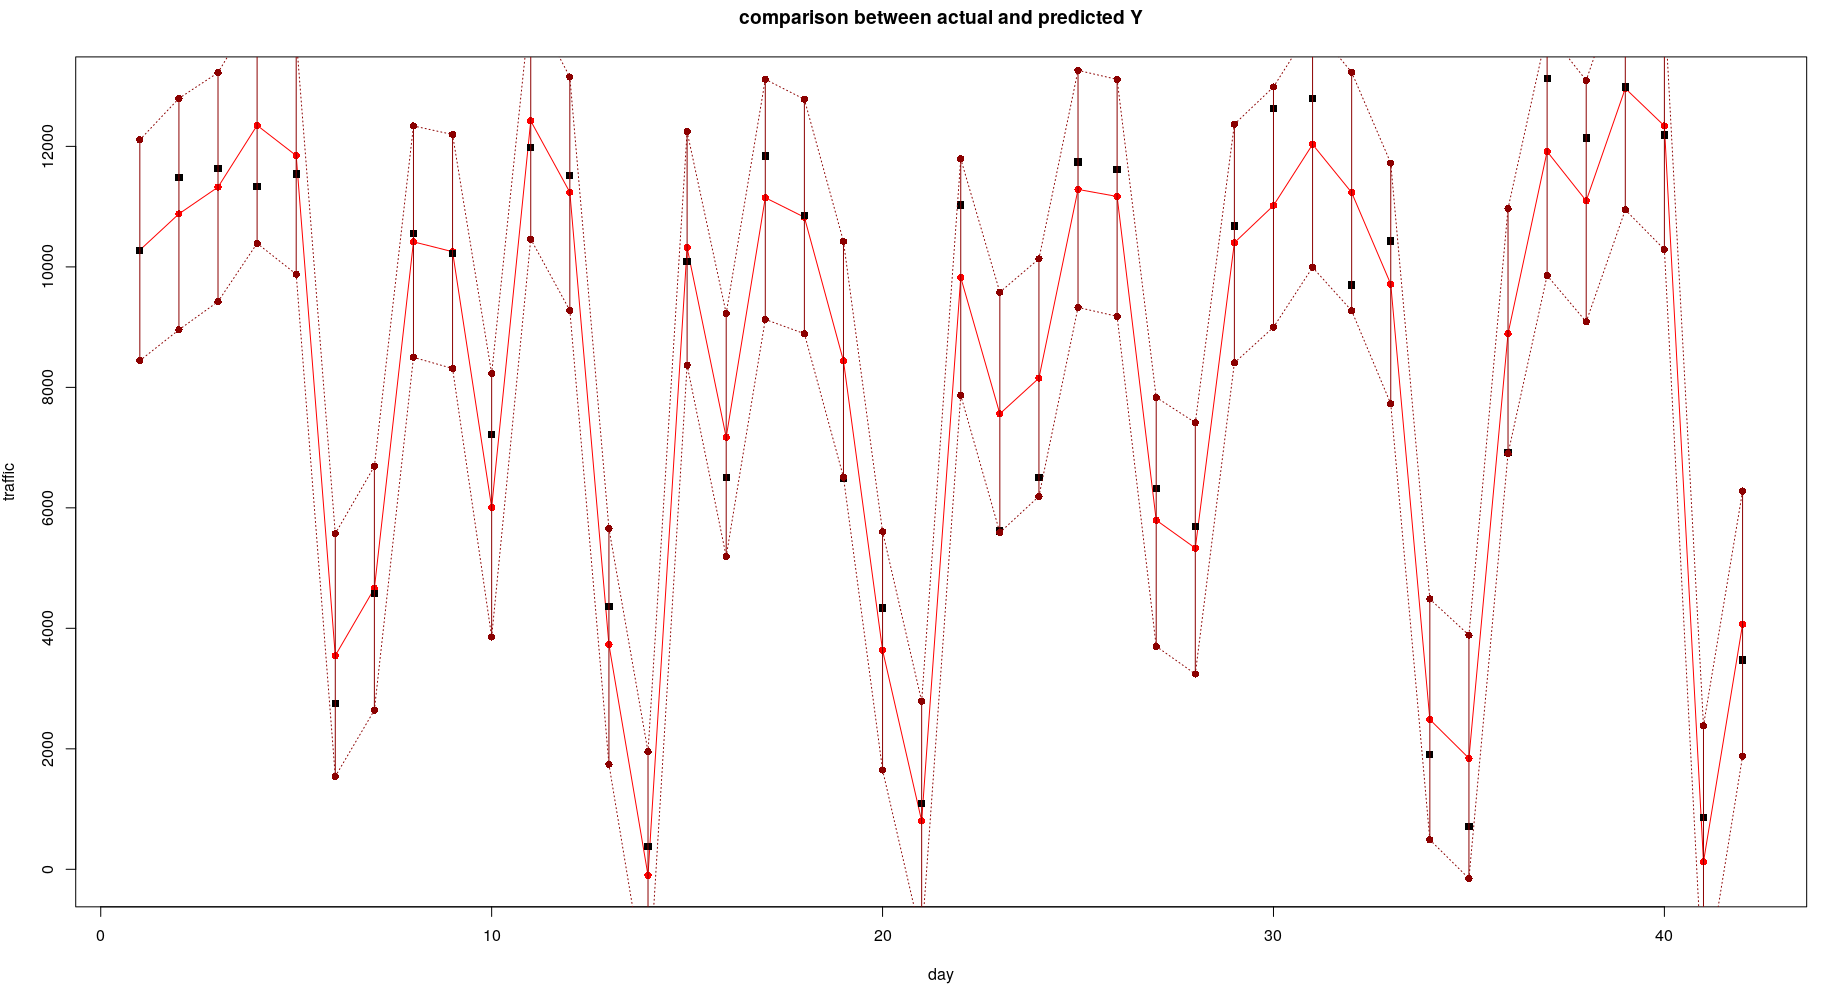
\includegraphics[width=100 mm]{pictures/m2_g2.png}
	\caption{90\% \alert{credibility intervals} in dark red, in black the true responses $ y $}
	\label{fig:M2_p2}
\end{figure}
\end{frame}

\begin{frame}{Without temperature}
\begin{figure}[H]
		\centering
	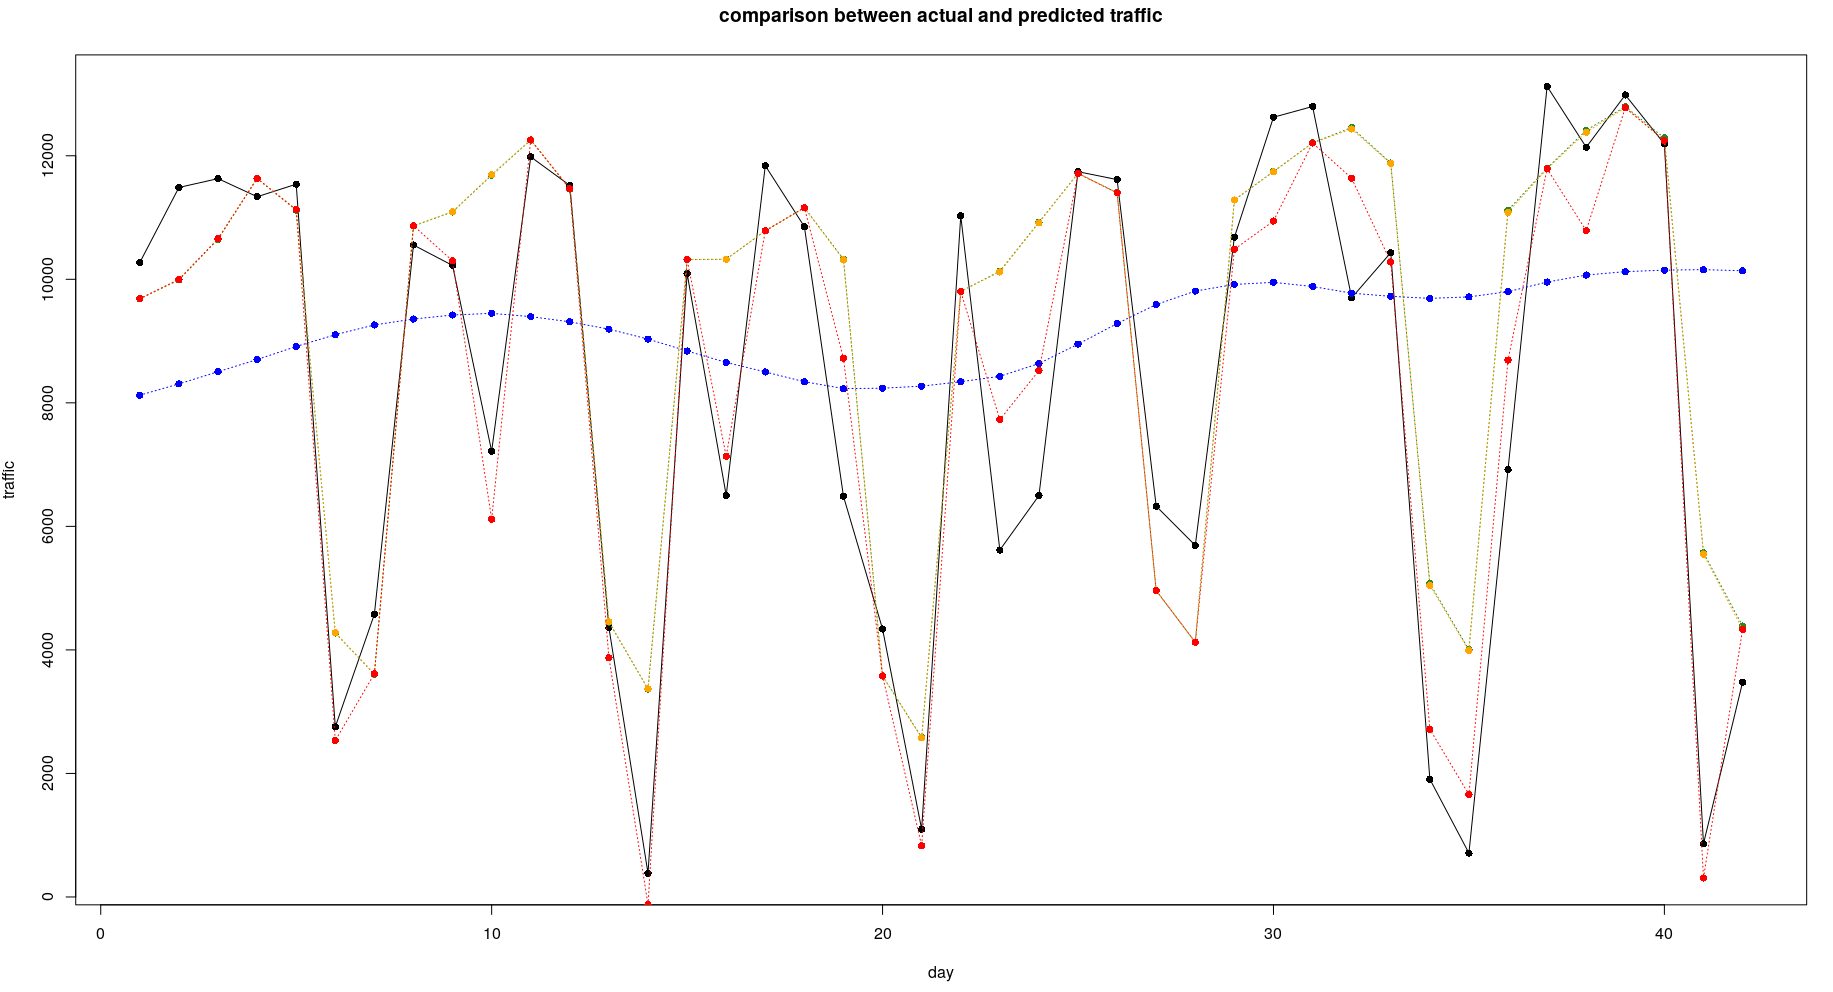
\includegraphics[width=100 mm]{pictures/m3_p1.png}
	\caption{Sum of trend (blue), periodicity (green), autoregression (yellow) and regression (red)}
	\label{fig:M3_p1}
\end{figure}
\end{frame}

\begin{frame}{Robust version}
We apply the \alert{lag operator} $\mathcal{L}_t(\cdot) = \frac{1}{2}(\cdot)_{t-1} + \frac{1}{3}(\cdot)_{t-S} +\frac{1}{6}(\cdot)_{t-2S}$ to the trend.

\begin{figure}[H]
	\centering
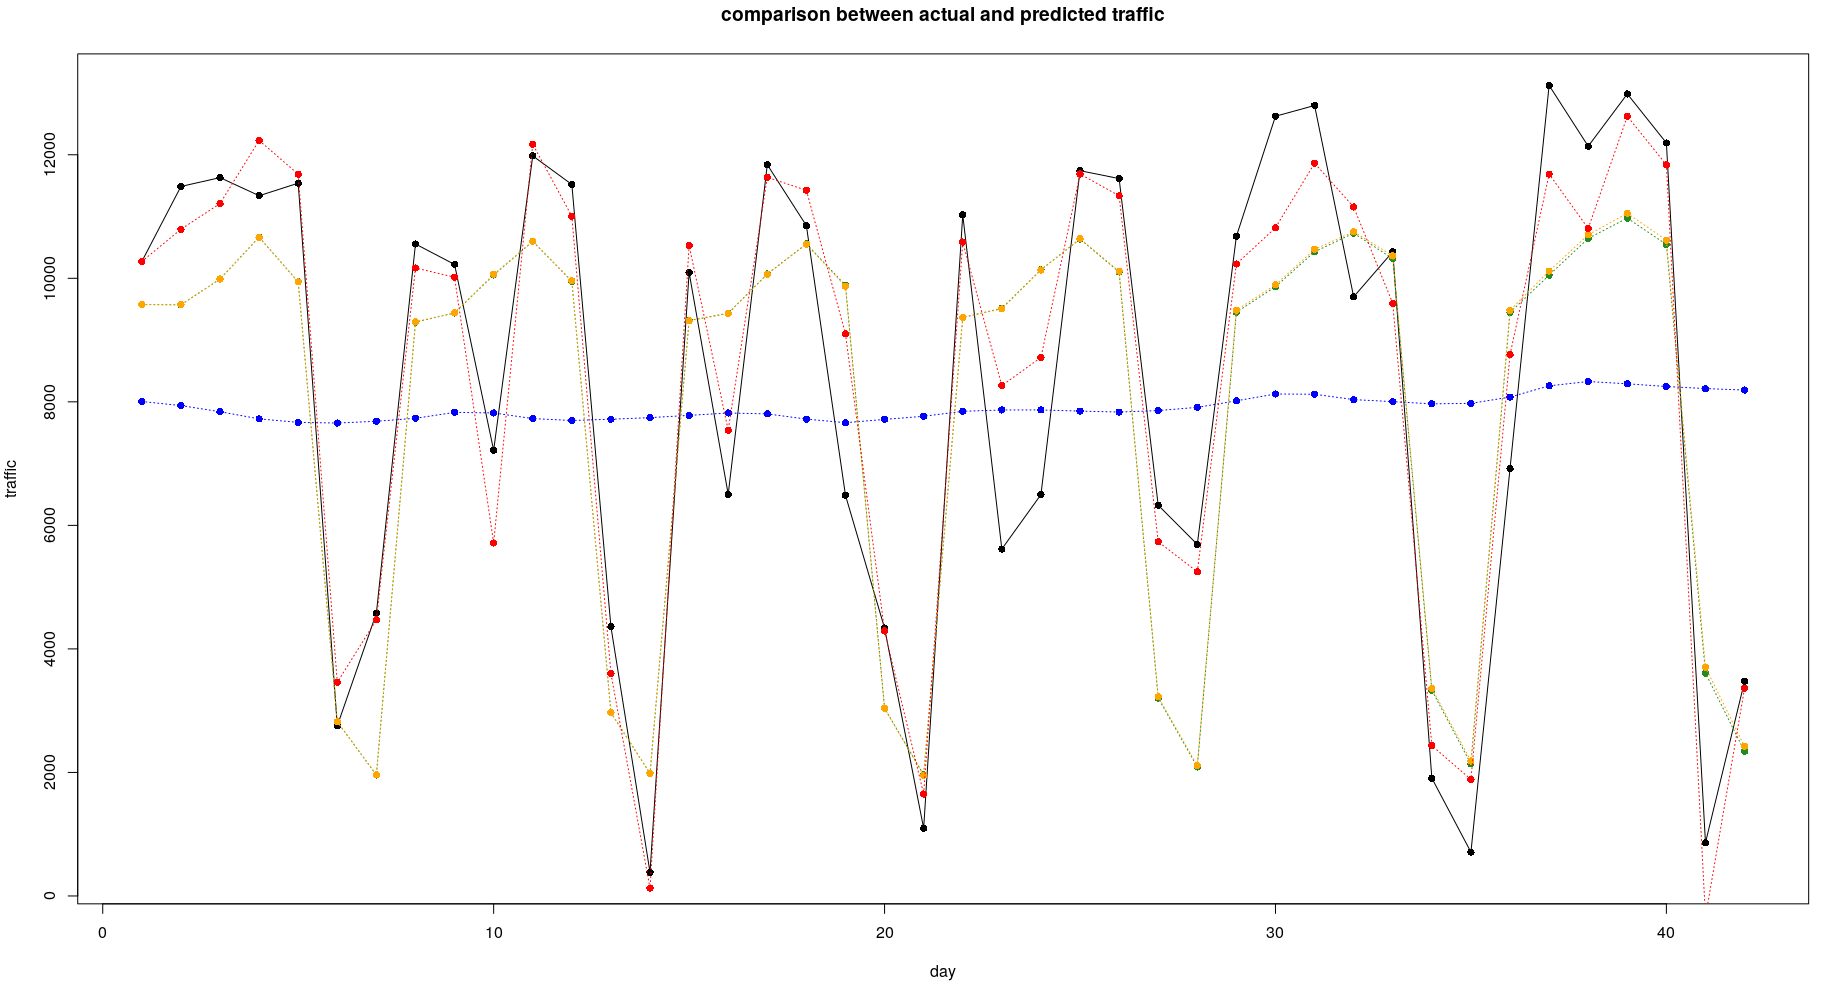
\includegraphics[width=100 mm]{pictures/m4_p1.png}
\caption{\tiny Cumulative action of trend (blue), periodicity (green), autoregression (yellow) and regression (red) in robust model}
\label{fig:M4_p1}
\end{figure}
\end{frame}

\begin{frame}{Evaluation of multiple  BSTS}
According to the criteria we have the following \alert{results}:
\tiny
\begin{table}[!htb]
	\centering
	\begin{tabular}{|c|c|c|c|}
		\hline
		& standard & no temperature & robust \\
		\hline
		Mean standardized residuals &$  0.5809041 $ & $  0.6066627 $ &$  0.6031869 $\\
		\hline
		Mean tail probabilities &$ 0.2979543 $ & $  0.298591 $ &$  0.2908414 $\\
		\hline
		$ elpd_{loo} $ &$ -362.6 $ & $  -365.4 $ &$  -364.1 $\\
		\hline
	\end{tabular}
\end{table}
\end{frame}

\begin{frame}{Future prediction}
We try to predict  \alert{one week ahead}
\begin{figure}[H]
	\centering
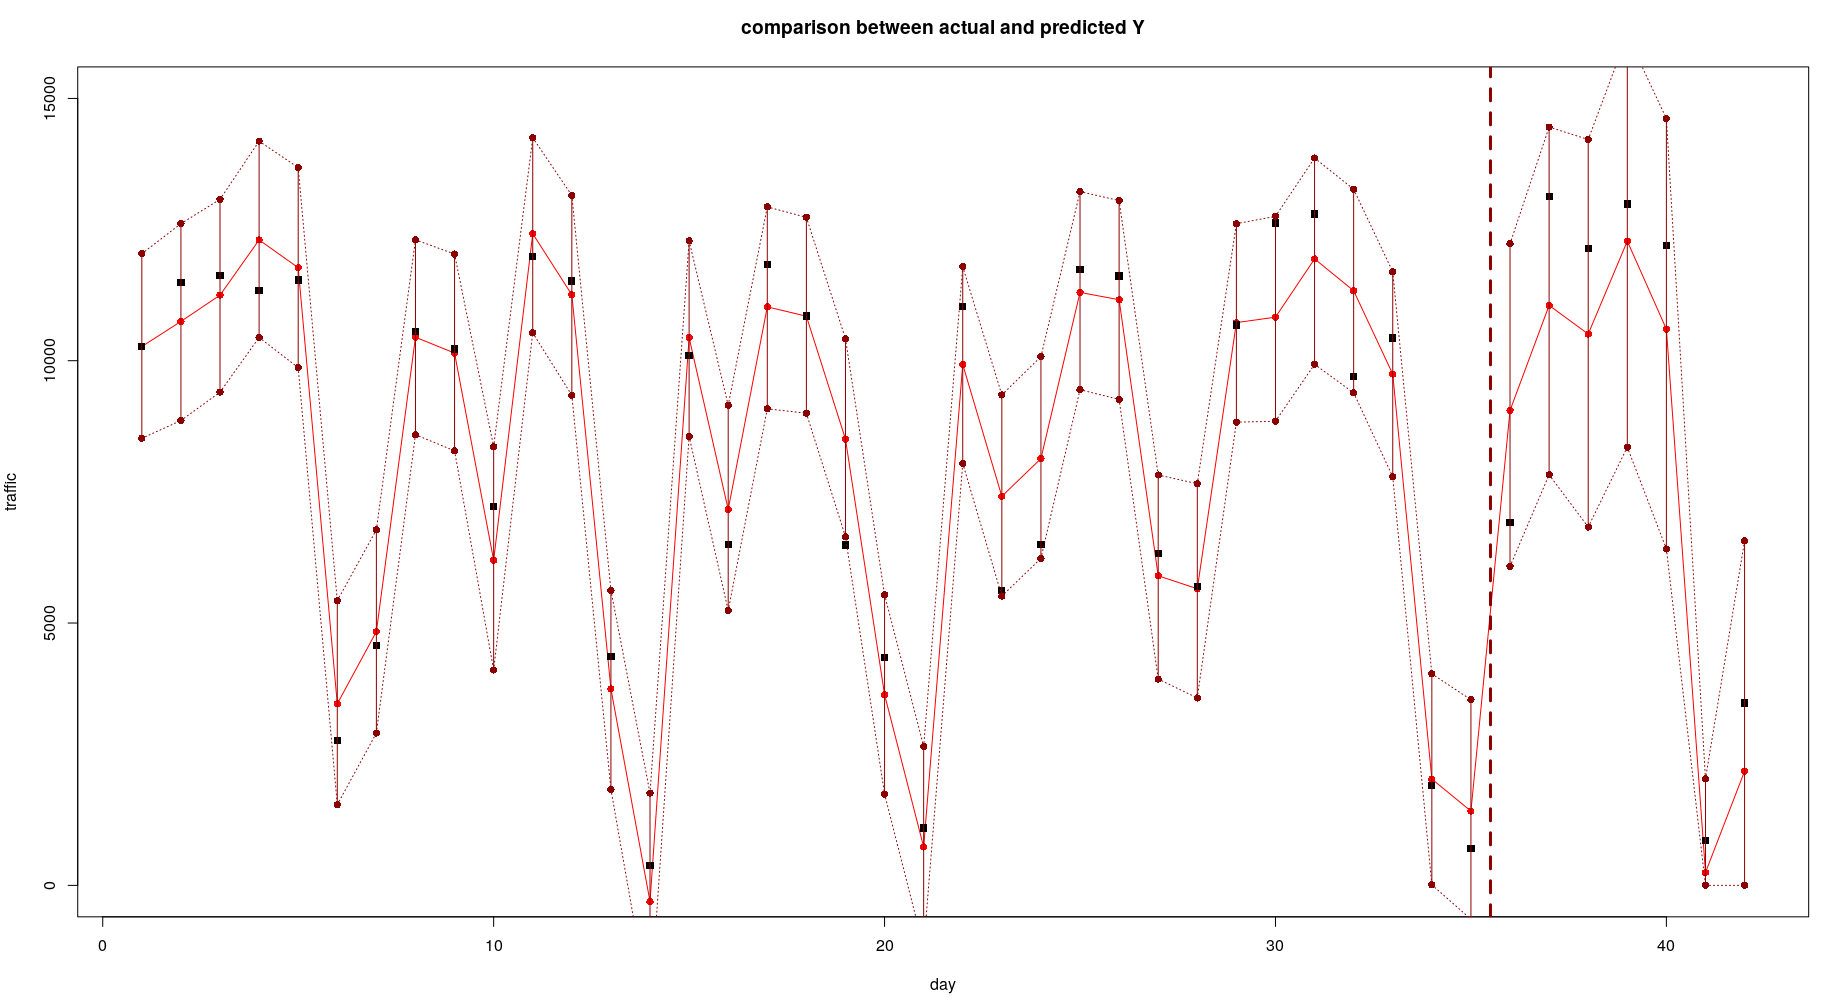
\includegraphics[width=100 mm]{pictures/predicted_traffic.png}
\caption{Predicted traffic with the model}
\label{fig:pt}
\end{figure}
\end{frame}

\begin{frame}{Standard BSTS with time zones}
\tiny

 	\begin{equation*}
\begin{aligned}
&\textsc{Model}\\
&Y_{F(t-1)+h} =
\mu_{t} + \gamma_{t} + \chi_{F(t-1)+h} +\\&\quad\quad+ \boldsymbol{\beta}^T\mathbf{z}_{th} + \tau_\epsilon^{-\frac{1}{2}}\tilde{\epsilon}_{F(t-1)+h}\\
&\mu_t = \mu_{t-1} + \delta_{t-1} +\tau_\eta^{-\frac{1}{2}}\tilde{\eta}_t\\
&\delta_t = \delta_{t-1} + \tau_v^{-\frac{1}{2}}\tilde{v}_t\\
&\gamma_t = \sum_{i=1}^{S-1}\gamma_{t+i-S} + \tau_w^{-\frac{1}{2}}\tilde{w}_t\\
&\chi_{F(t-1)+h} = \sum_{j=1}^{F-1}\chi_{F(t-1)+h+j-F} +\\&\quad\quad+ \tau_u^{-\frac{1}{2}}\tilde{u}_{F(t-1)+h}\\
&\tilde{\epsilon}_{F(t-1)+h}, \tilde{\eta}_t, \tilde{v}_t, \tilde{w}_t, \tilde{u}_{F(t-1)+h} \overset{iid}{\sim} \mathcal{N}(0,1)\\
\\
&\textsc{Initial Conditions}\\
&\mu_0 \sim \mathcal{N}(m, \tau_\eta)\quad \quad\quad\quad \quad \quad \quad\  m\ \ hpm\\
&\delta_0 \sim \mathcal{N}(d, \tau_v)\quad \quad\quad\quad \quad \quad \quad \quad d\ \ \ hpm\\
&\boldsymbol{\gamma}_{0:(2-S)} \sim \mathcal{N}_{S-1}(\mathbf{g}, \tau_w\mathbf{I})\quad\ \ \mathbf{g}\ \ hpm\\
&\boldsymbol{\chi}_{0:(2-F)} \sim \mathcal{N}_{F-1}(\mathbf{c}, \tau_u\mathbf{I})\quad\ \  \mathbf{c}\ \ hpm\\
\\
\end{aligned}
\qquad \qquad
\begin{aligned}[c]
&\textsc{Priors}\\
&\boldsymbol{\beta} \sim \mathcal{N}_p(\mathbf{0}, \tau_b \mathbf{I})\ \ \quad \quad \quad \quad \quad \tau_b\ \quad \ hpm\\
&\tau_\epsilon \sim Unif(a_\epsilon, b_\epsilon)\quad\quad\ \quad \quad a_\epsilon, b_\epsilon\ \ hpm\\
&\tau_\eta \sim Unif(a_\eta, b_\eta)\quad\quad\quad \quad a_\eta, b_\eta\ \ hpm\\
&\tau_v \sim Unif(a_v, b_v)\quad\quad\quad \quad a_v, b_v\ \ hpm\\
&\tau_w\sim Unif(a_w, b_w)\quad\quad\quad a_w, b_w\ \ hpm\\
&\tau_u\sim Unif(a_u, b_u)\quad\quad\quad\ \ a_u, b_u\ \ hpm\\
&\\
&\\
&\\
&\\
&\\
&\\
&\textsc{Independence}\\
&\{\tilde{\epsilon}_t, \tilde{\eta}_t, \tilde{w}_t, \tilde{v}_t, \mu_0, \delta_0, \boldsymbol{\gamma}_{0:(-S+2)}, \\&\boldsymbol{\chi}_{0:(2-F)}, \boldsymbol{\beta}, \tau_\epsilon, \tau_\eta, \tau_v, \tau_w, \tau_u \}\\ &family\ of \independent real\ random\ variables\\
&\\
&\\
\end{aligned}
\end{equation*}
\end{frame}

\begin{frame}{Division in time zones}
\begin{figure}[H]
	\centering
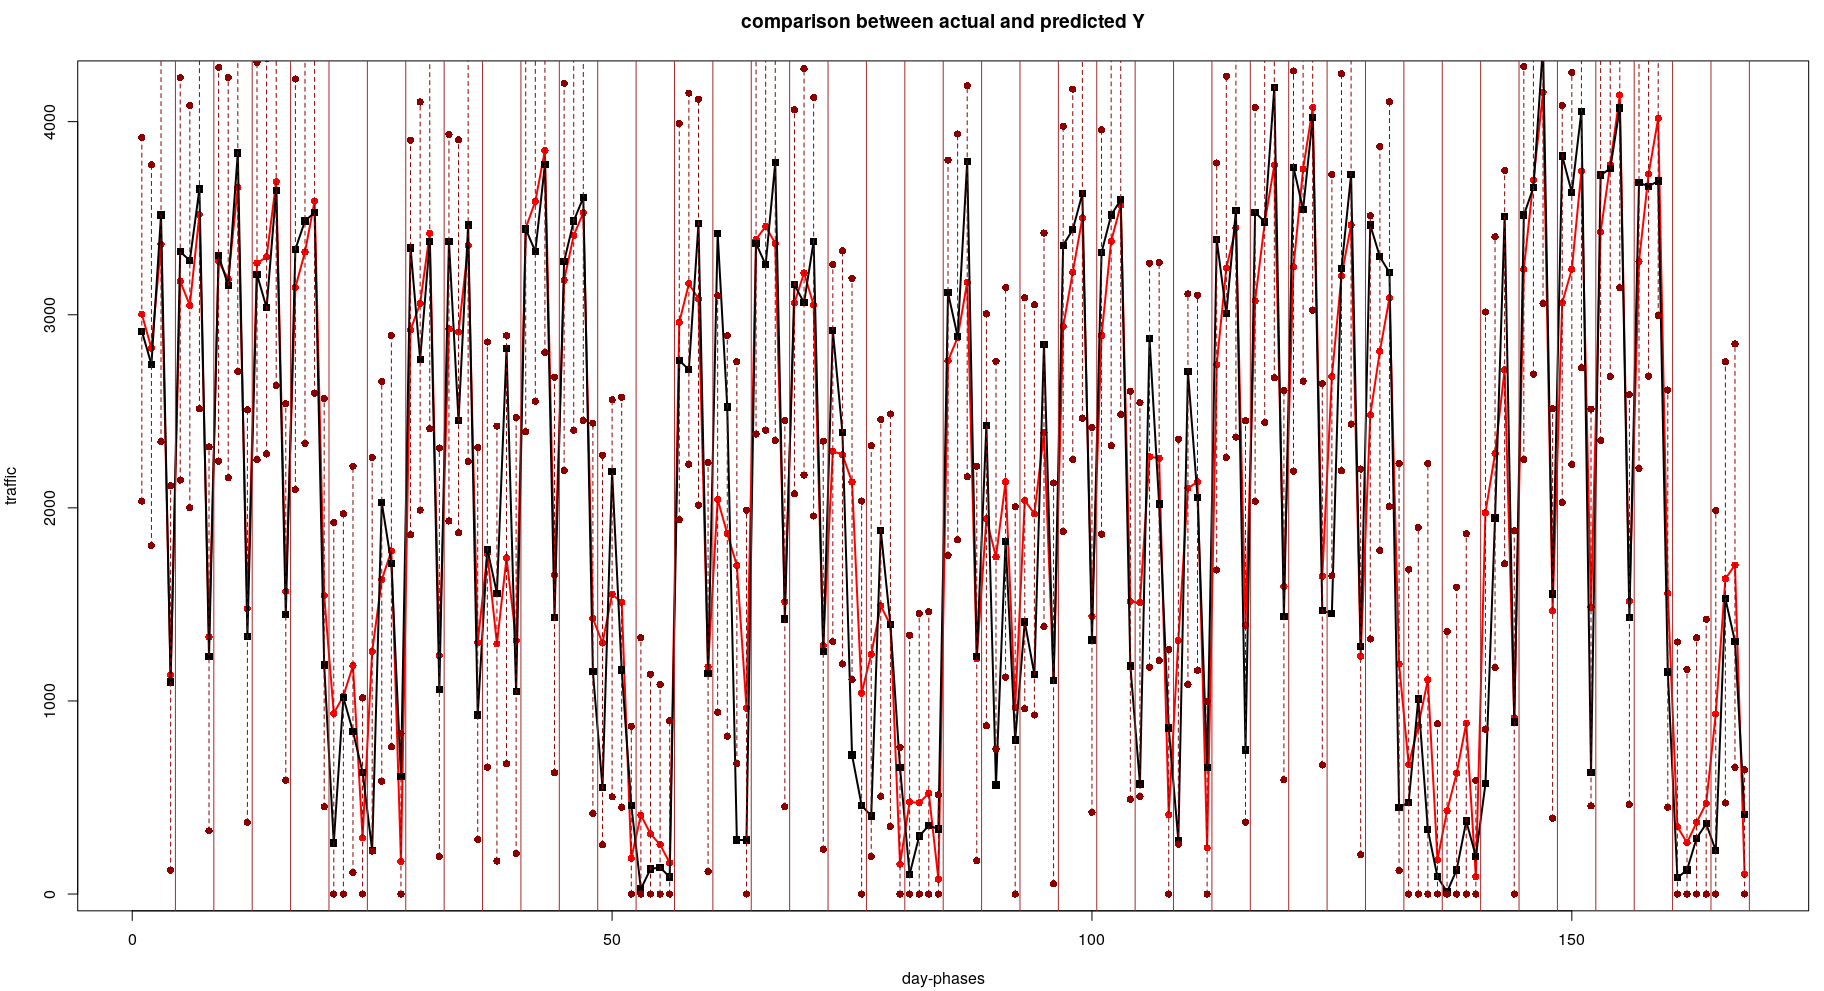
\includegraphics[width=100 mm]{pictures/Time_series.png}
\caption{Global time series per slot}
\label{fig:time series}
\end{figure}
\end{frame}

\begin{frame}{Network models}
In the network models we deal with the \alert{flows} of bicycles inward and outward a cluster of station, given a time interval.\\

The problem is the with the very high dimensionality of the data, and the computational weight due to the high number of parameters.\\

To shrink the model we first introduced a prior clusterization with a modified \alert{DBSCAN} and later using simplifying hypothesis. 
\end{frame}

\begin{frame}{Modified DBSCAN}
The euclidian distance isn't versatile enough
\begin{itemize}
	\item We fed the classic DBSCAN a different \alert{semidistance}, $ smd(x,y) = \frac{p(y)+p(x)}{2}||x-y|| $.
	\item $p(x) = g(||x-x_0||)$ where $x_0$ are the coordinates of the Duomo, and $g(u) = \max\{\beta, e^{(\frac{u}{\alpha})^2\log{(1-\gamma)}}+\gamma\}$ 
	\item We fitted the parameters in a way to minimize the autorings, and to break down the biggest clusters
\end{itemize}
\end{frame}

\begin{frame}
\begin{columns}
	\begin{column}{.5\linewidth}
		\begin{figure}[H]
			\centering
			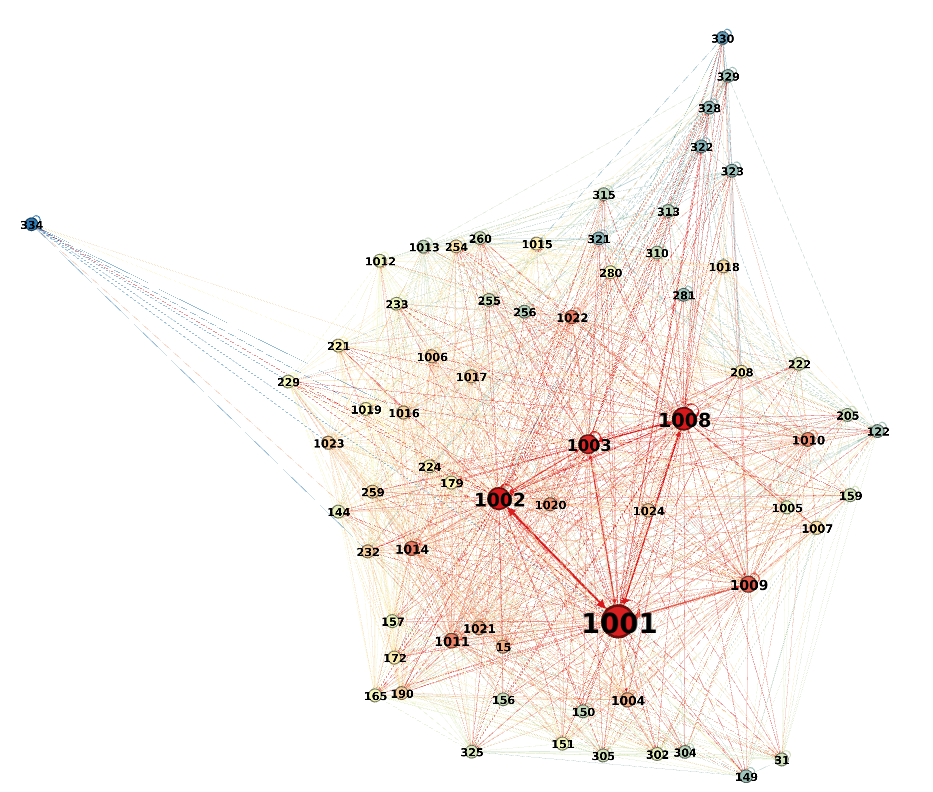
\includegraphics[width=1\linewidth]{pictures/old_model_gephi.png} 
		\end{figure}
	\end{column}
\begin{column}{.5\linewidth}
\begin{figure}[H]
	\centering
	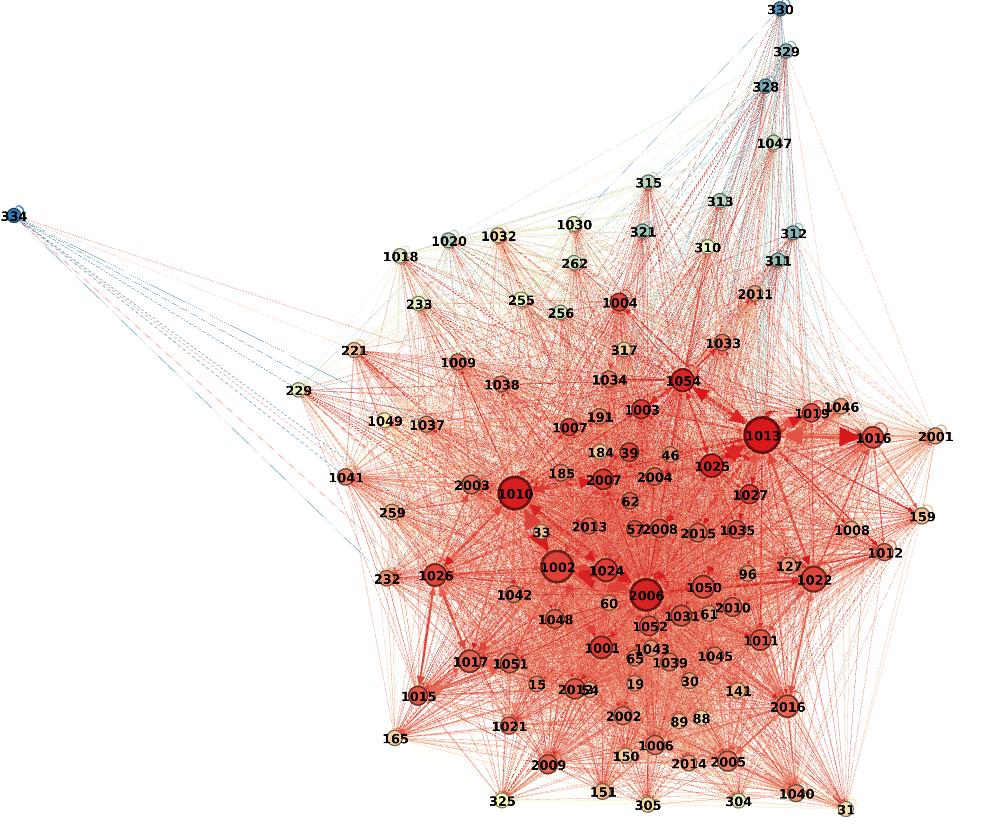
\includegraphics[width=1\linewidth]{pictures/new_model_gephi.png} 
\end{figure}

\end{column}
\end{columns}
\end{frame}

\begin{frame}{Preprocessing}
\begin{columns}
	\begin{column}{.5\linewidth}
		\begin{figure}[H]
			\centering
			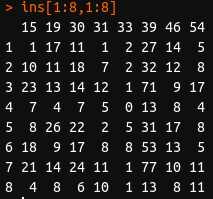
\includegraphics[width=.8\linewidth]{pictures/ins_with_header.png} 
		\end{figure}
	\end{column}
	\begin{column}{.5\linewidth}
		The two flows are structured as 168 x 109 matrices where the columns are the nodes and the rows are the evolving time
	\end{column}
\end{columns}
\alert{Correlations} between the flows in the same node
\begin{figure}[H]
	\centering
	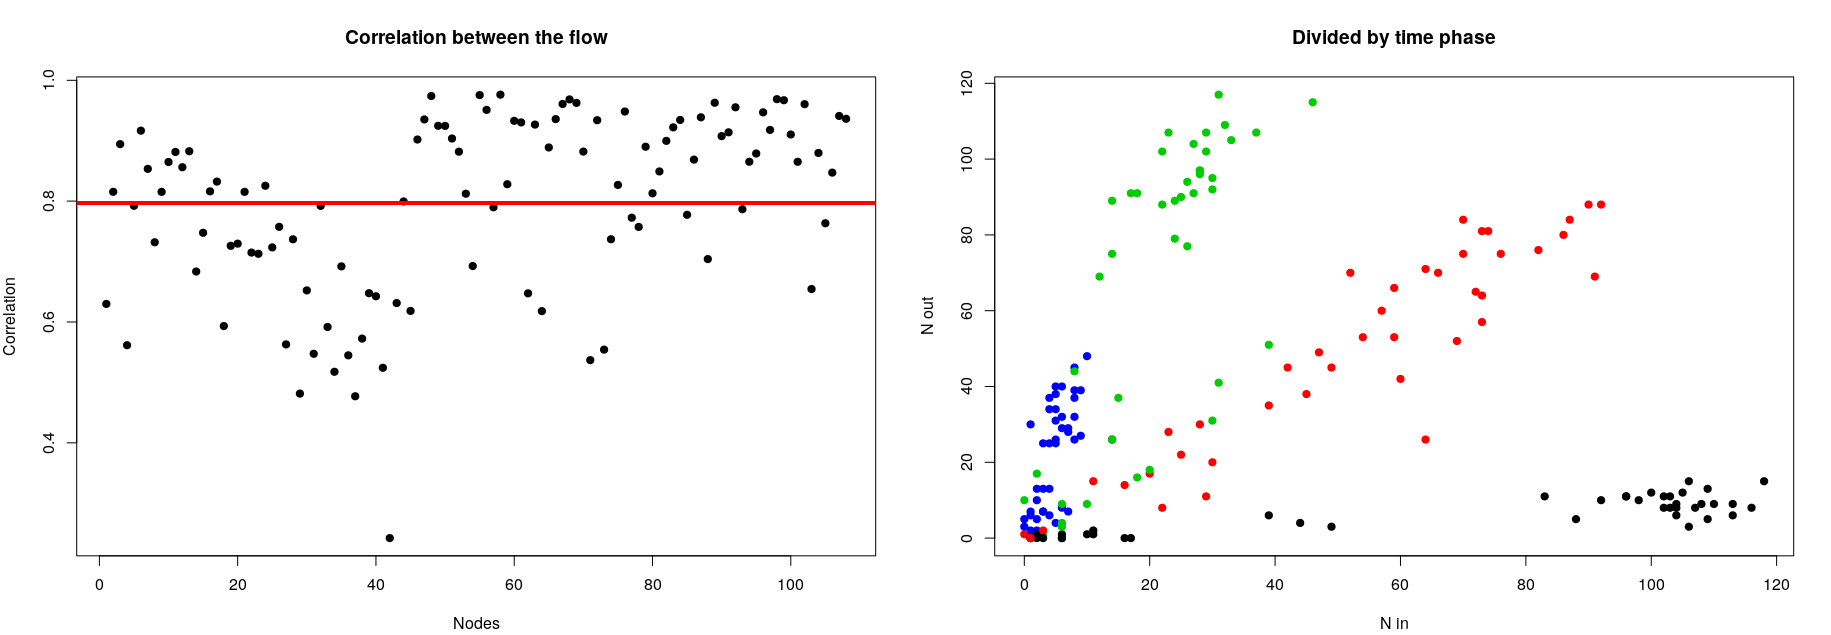
\includegraphics[width=1\linewidth]{pictures/correlation_pres.png} 
\end{figure}
\end{frame}

\begin{frame}{Bivariate Poisson}
The likelihood is a \alert{Bivariate Poisson}, a distribution over $\mathbb{N}\times\mathbb{N}$.
\begin{equation}
\begin{cases}
Y_j = X_0 + X_j \quad j = 1,2\\
X_j \sim \mathrm{Po}(\lambda_j) \quad j = 0,1,2
\end{cases}
\end{equation}
In this way $\mathrm{Cov}(Y_1, Y_2) = \mathrm{Var}(X_0) = \lambda_0$. And marginally $Y_j \sim \mathrm{Po}(\lambda_0 + \lambda_j)$.
\end{frame}

\begin{frame}{Some simplifying hypothesis}
\begin{equation*}
\begin{aligned}
&\textsc{Two way mixed effect}\\
&\beta_{ith}\cdot\mathbf{x} \Rightarrow (\alpha_{t} + \gamma_{h})\cdot\mathbf{x}\\
&\\
&\textsc{Offsets}\\
&\log(\frac{\lambda_{ith}}{O_i}) = (\alpha_{t} + \gamma_{h})\cdot\mathbf{x} \\&\Rightarrow \log(\lambda_{ith}) = \log(O_i) + (\alpha_{t} + \gamma_{h})\cdot\mathbf{x}\\
&\\
\end{aligned}
\end{equation*}
\end{frame}

\begin{frame}{The offsets model}
\begin{equation}
\begin{cases}
\log(\lambda^{(j)}_{ith}) = (\boldmath{\theta^{(j)} +  \alpha^{(j)}_{t} + \gamma_{h}^{(j)})}\cdot\mathbf{x} + \log(O_i)\\
\theta^{(j)}|a,B \stackrel{iid}{\sim} \mathcal{N}(a,B)\\
\alpha_{t}^{(j)}|\Sigma \stackrel{iid}{\sim} \mathcal{N}(0, \Sigma)\\
\gamma_{h}^{(j)}|\Omega \stackrel{iid}{\sim} \mathcal{N}(0, \Omega)\\
a \sim \mathcal{N}(a_0, A_0)\\
B \sim invWishart(B_0, p+1)\\
\Sigma, \Omega \stackrel{iid}{\sim} invWishart(C_0, p+1)

\end{cases}
\end{equation}

Where $\alpha_{t}^{(j)}, \beta_{h}^{(j)}, \theta^{(j)}, a \in \mathbb{R}^3$, $\Sigma, \Omega, B \in \mathbb{R}^{3\times 3}$ are the parameters, $A_0, B_0, C_0 \in \mathbb{R}^{3\times 3},\quad a_0 \in \mathbb{R}^3$ are the hyperparameters, and $\mathbf{x}$ are the covariates.\\

The offsets are the the average of the traffic of the first 12 days.
\end{frame}

\begin{frame}{The parametric offsets (PO) model}
The offsets are now grouped with the other parameters.
\begin{equation}
\begin{cases}
\log(\lambda^{(j)}_{ith}) = (\boldmath{\theta^{(j)} +  \alpha^{(j)}_{t} + \beta_{h}^{(j)})}\cdot\mathbf{x} + \Phi_i\\
\theta^{(j)}|a,B \stackrel{iid}{\sim} \mathcal{N}(a,B)\\
\alpha_{t}^{(j)}|\Sigma \stackrel{iid}{\sim} \mathcal{N}(0, \Sigma)\\
\beta_{h}^{(j)}|\Omega \stackrel{iid}{\sim} \mathcal{N}(0, \Omega)\\
\Phi_i \stackrel{iid}{\sim} \mathcal{N}(\Phi_0, F_0)\\
a \sim \mathcal{N}(a_0, A_0)\\
B \sim invWishart(B_0, p+1)\\
\Sigma, \Omega \stackrel{iid}{\sim} invWishart(C_0, p+1)

\end{cases}
\end{equation}

Where $\alpha_{t}^{(j)}, \beta_{h}^{(j)}, \theta^{(j)}, a \in \mathbb{R}^3$, $\Sigma, \Omega, B \in \mathbb{R}^{3\times 3}$, $\Phi_i \in \mathbb{R}$ are the parameters, $A_0, B_0, C_0, F_0 \in \mathbb{R}^{3\times 3},\quad a_0 \in \mathbb{R}^3, \Phi_0 \in \mathbb{R}$ are the hyperparameters, and $\mathbf{x}$ are the covariates.
\end{frame}

\begin{frame}{Posterior with JAGS}
\begin{columns}
	\begin{column}{.5\linewidth}
		\begin{figure}[H]
			\centering
			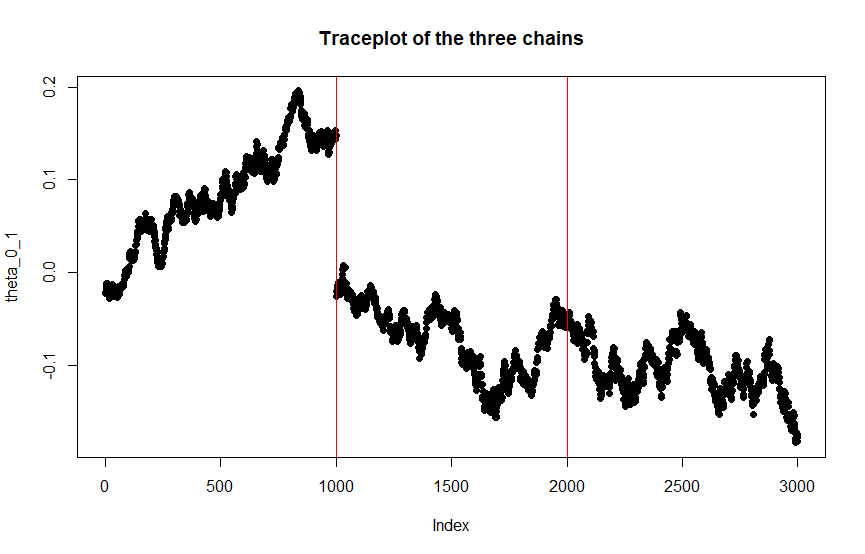
\includegraphics[width=1\linewidth]{pictures/three_chains.png} 
		\end{figure}
		\begin{tabular}{ |c|c|c| } 
			\hline
			& $N^{IN}$ & $N^{OUT}$ \\ 
			\hline
			Offsets & 41.0\% & 62.2\% \\ 
			PO & 39.7\% & 38.6\% \\ 
			\hline
		\end{tabular}
	\end{column}
	\begin{column}{0.5\linewidth}
		\begin{figure}[H]
			\centering
			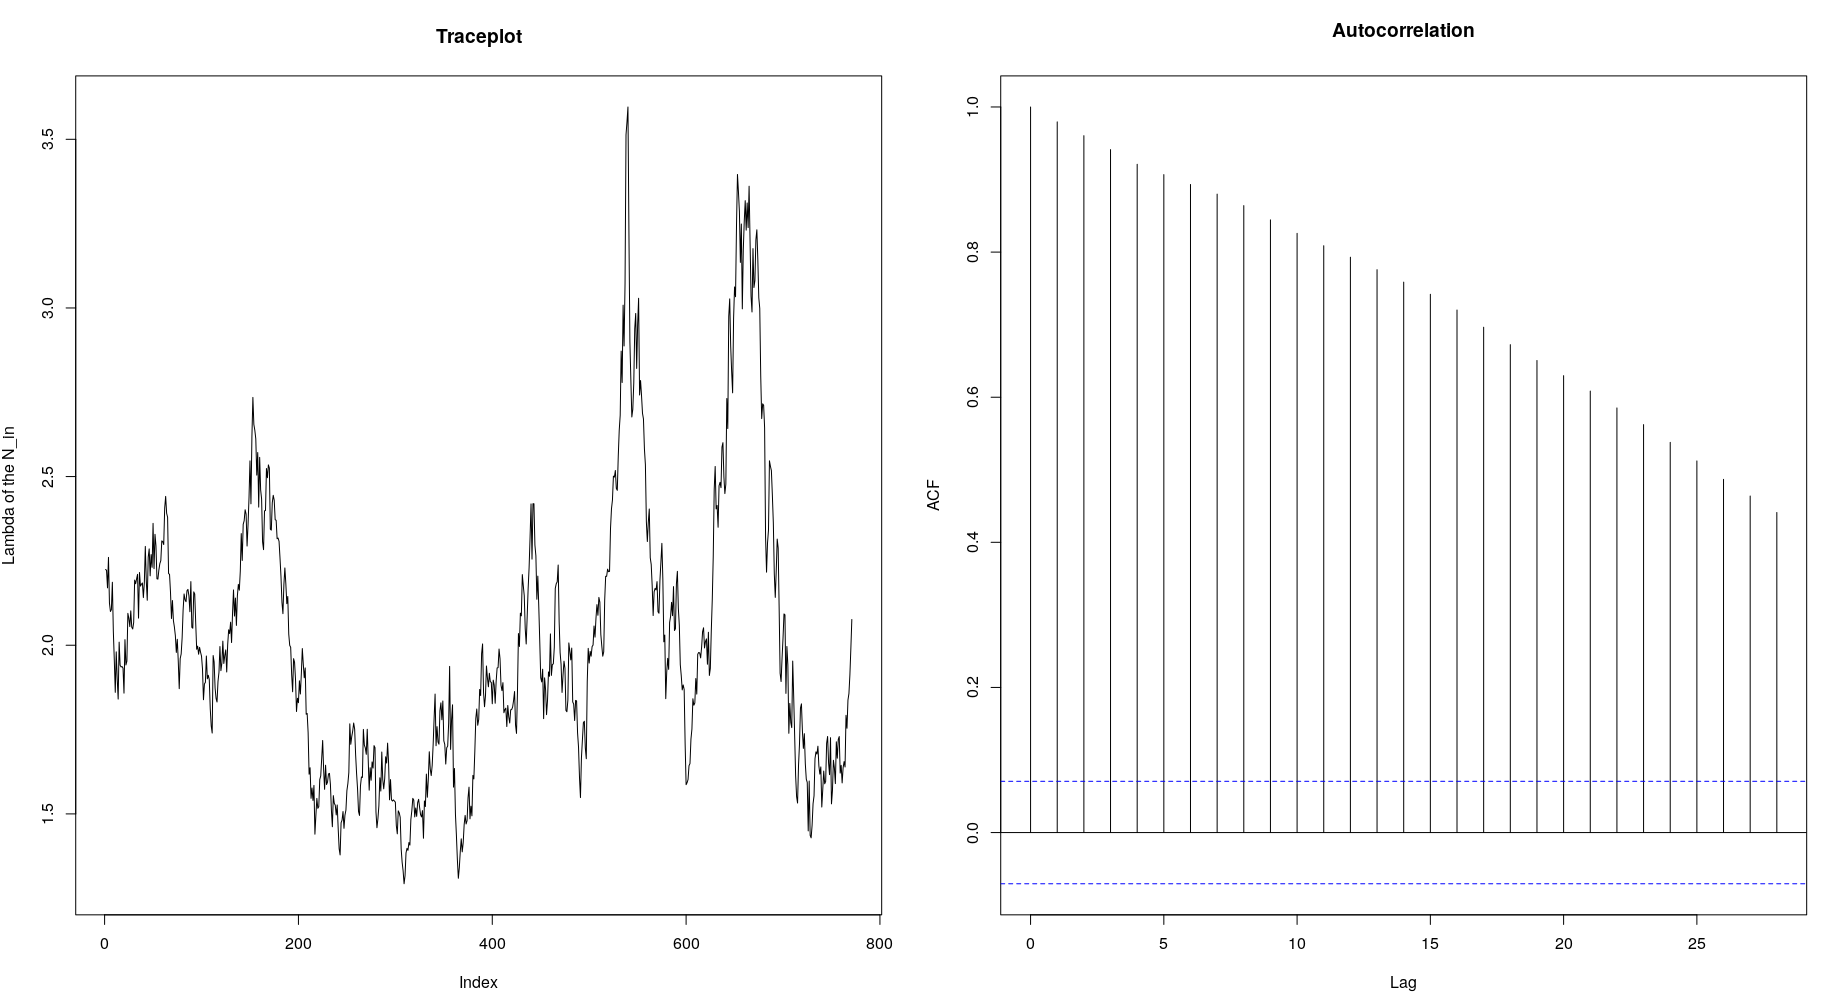
\includegraphics[width=1\linewidth]{pictures/posterior_off.png} 
		\end{figure}
		The results are unsatisfactory, the iterations are not enough to stabilize the MCMC and the autocorrelation is too high. The \alert{predictive power} is low.
	\end{column}
\end{columns}
\end{frame}

\begin{frame}
\begin{figure}[H]
\centering
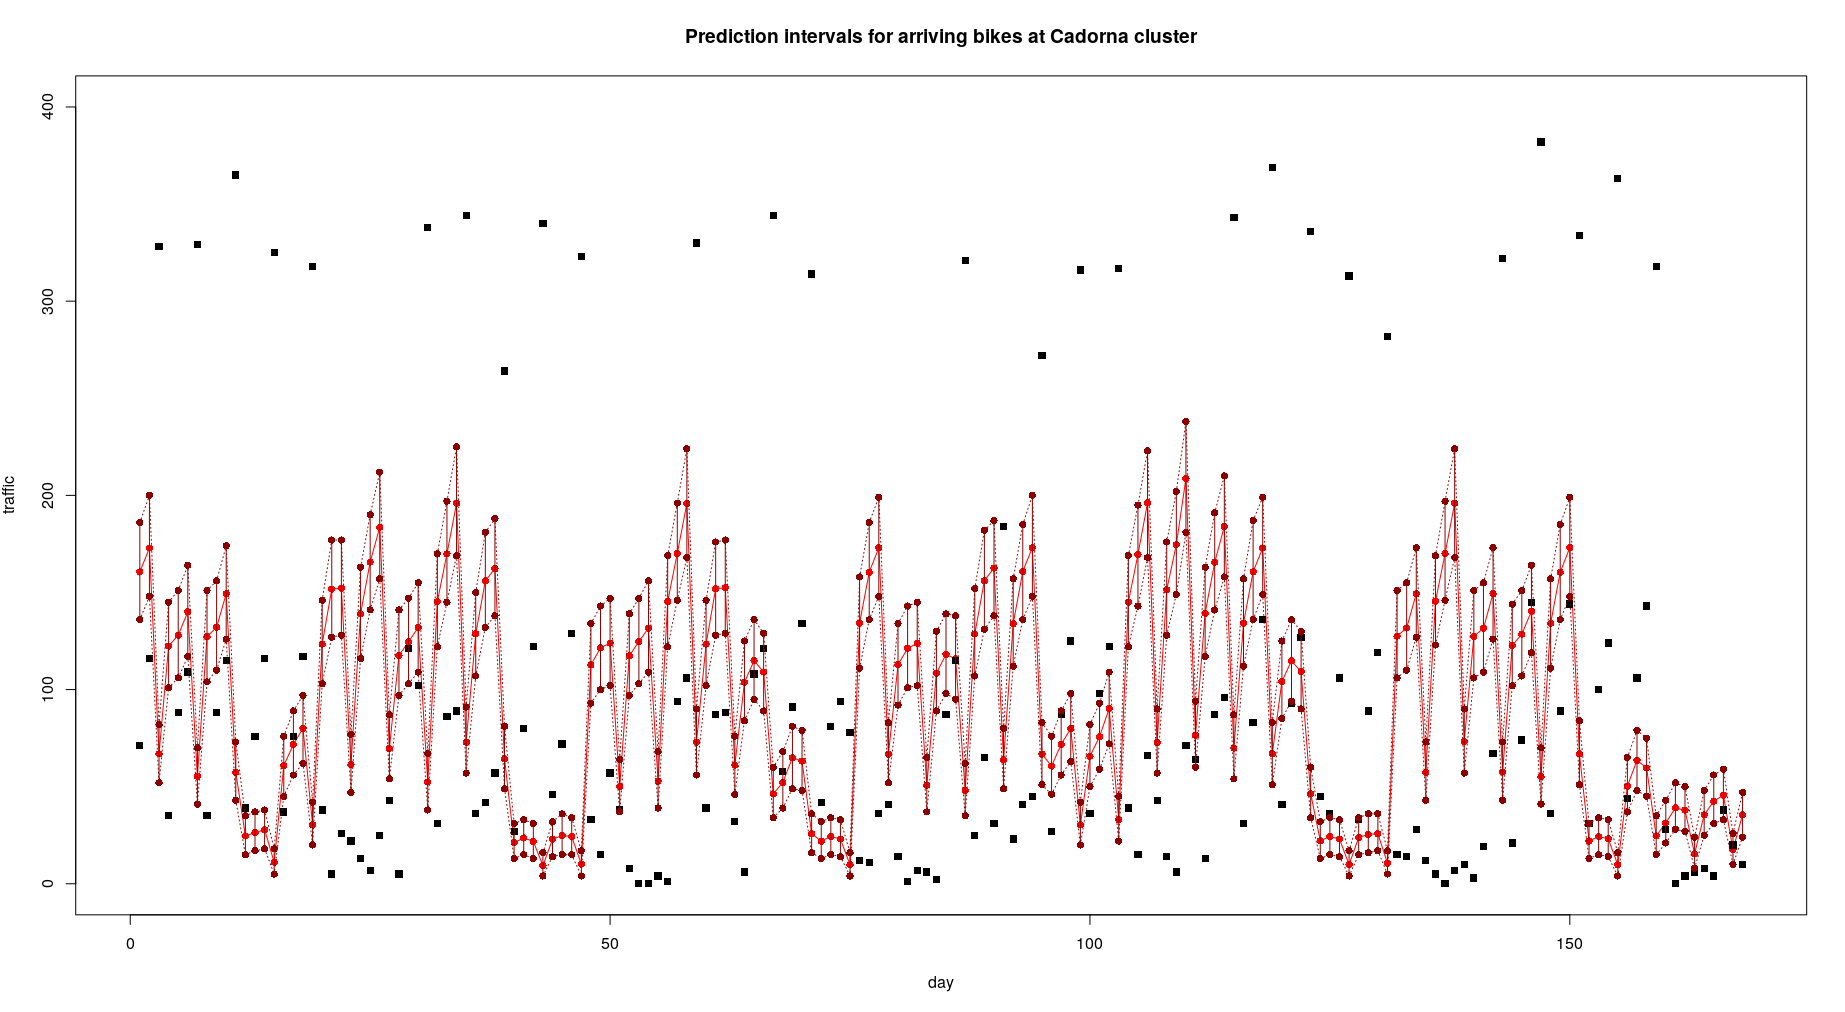
\includegraphics[width=1\linewidth]{pictures/cadorna_nin.png} 
\end{figure}
\end{frame}

\end{document}

